%!TEX root = ../MasterThesis.tex

\chapter{Design of a collaborative system} % (fold)
\label{cha:system_design}

This chapter is about the design of a collaborative system that supports the investigation of \gls{E-commerce} fraud incidents. It starts with a discussion of the semantics of the underlying \gls{RDF} data sets, and how these can be combined across various organizations. After that it shows how these information can be provided by the relevant participants based on the \gls{E-commerce} fraud investigation scenario described in Chapter~\ref{cha:context_analysis}. For this purpose it looks in detail into the partially centralized \gls{P2P} communication architecture, and shows how that can be used for securely sharing the relevant information between the stakeholders.

% sub chapter selecting a data schema
%!TEX root = ../MasterThesis.tex

\section{\gls{RDF} vocabularies and Web Ontologies for \gls{E-commerce}}
\label{sec:choose_data_schema}

As a major objective of the \gls{E-commerce} fraud investigation system is to collect the various transactional information from online merchants, \gls{PSP}s and issuers, combine and link them together, as well as analyse the resulting data set from different view points to find abnormal activities, the information exchanged between the relevant participants either have to follow commonly available \gls{RDF} vocabularies, have to be based on a custom shared \gls{RDF} vocabulary that has been specifically designed for this system, or have to be mapped and linked against each other from different \gls{RDF} schema specifications.

\subsection{Reuse of common \gls{RDF} vocabularies}
\label{subsec:reuse_vocab_web}

One valid approach to come up with a data schema for the collaborative system is to take a look into commonly used \gls{RDF} vocabularies and Web ontologies, and try to figure out whether they can be used for describing the information that need to be exchanged between participants of the \gls{E-commerce} fraud investigation system. When consulting the Semantic Web community for commonly agreed upon and highly used \gls{RDF} schema specifications, one will come up with the following list (see Table~\ref{tab:used_vocab_rdf}):\@

\begin{table}[H]
\centering
\begin{tabular}{p{3cm}llp{4.5cm}}
\hline
\textbf{Name} & \textbf{Prefix} & \textbf{Describes} & \textbf{Namespace URI} \\
\hline
Dublin Core & dc: & Meta data & \url{http://purl.org/dc/terms/} \\
\hline
FOAF & foaf: & People & \url{http://xmlns.com/foaf/0.1/} \\
\hline
Geo & pos: & Positions & \url{http://www.w3.org/2003/01/geo/wgs84\_pos\#} \\
\hline
Geo Names & gn: & Locations & \url{http://www.geonames.org/ontology\#} \\
\hline
Good Relations & gr: & Products & \url{http://purl.org/goodrelations/v1\#} \\
\hline
RDF & rdf: & Core framework & \url{http://www.w3.org/1999/02/22-rdf-syntax-ns\#} \\
\hline
RDFS & rdfs: & RDF vocabularies & \url{http://www.w3.org/2000/01/rdf-schema\#} \\
\hline
Schema.org & schema: & Schema.org vocabularies & \url{http://schema.org/} \\
\hline
SKOS & skos: & Controlled vocabularies & \url{http://www.w3.org/2004/02/skos/core\#} \\
\hline
vCard & vcard: & Business Cards & \url{http://www.w3.org/2006/vcard/ns\#} \\
\hline
Web Ontology Language & owl: & Ontologies & \url{http://www.w3.org/2002/07/owl\#} \\
\hline
XML Schema Datatypes & xsd: & Data types & \url{http://www.w3.org/2001/XMLSchema\#} \\
\hline
\end{tabular}
\caption[Commonly used \gls{RDF} vocabularies on the Web]{Commonly used \gls{RDF} vocabularies on the Web \citep[pg. 41]{wood2014linked}}
\label{tab:used_vocab_rdf}
\end{table}

Based on these existing schema specifications describing a fictive consumer named ``Max Mustermann'' \gls{incl}\ his home address can be done by combining data utilizing the \gls{FOAF} and \gls{vCard} vocabularies into a \gls{RDF} data set such as described in Listing~\ref{lst:sample_customer_mustermann} and visualized as directed graph in Figure~\ref{fig:images_sample_customer}. The described resource is uniquely identified by the \gls{URI} \url{http://www.merchant1.com/customers/MaxMustermann}. Additionally, one can see that these vocabularies use expressive names for their entities and predicates, which make it easier to understand their intended meanings (e.g.\ ``foaf:givenname'', ``vcard:locality'', \ldots).  \@

\begin{listing}[H]
  \inputminted[linenos,
               numbersep=5pt,
               breaklines=true,
               frame=lines]{TURTLE}
               {./samples/sample_customer_mustermann.ttl}
  \caption{Personal related information about a fictive consumer in \gls{RDF}}
\label{lst:sample_customer_mustermann}
\end{listing}

\begin{figure}[H]
	\centering
		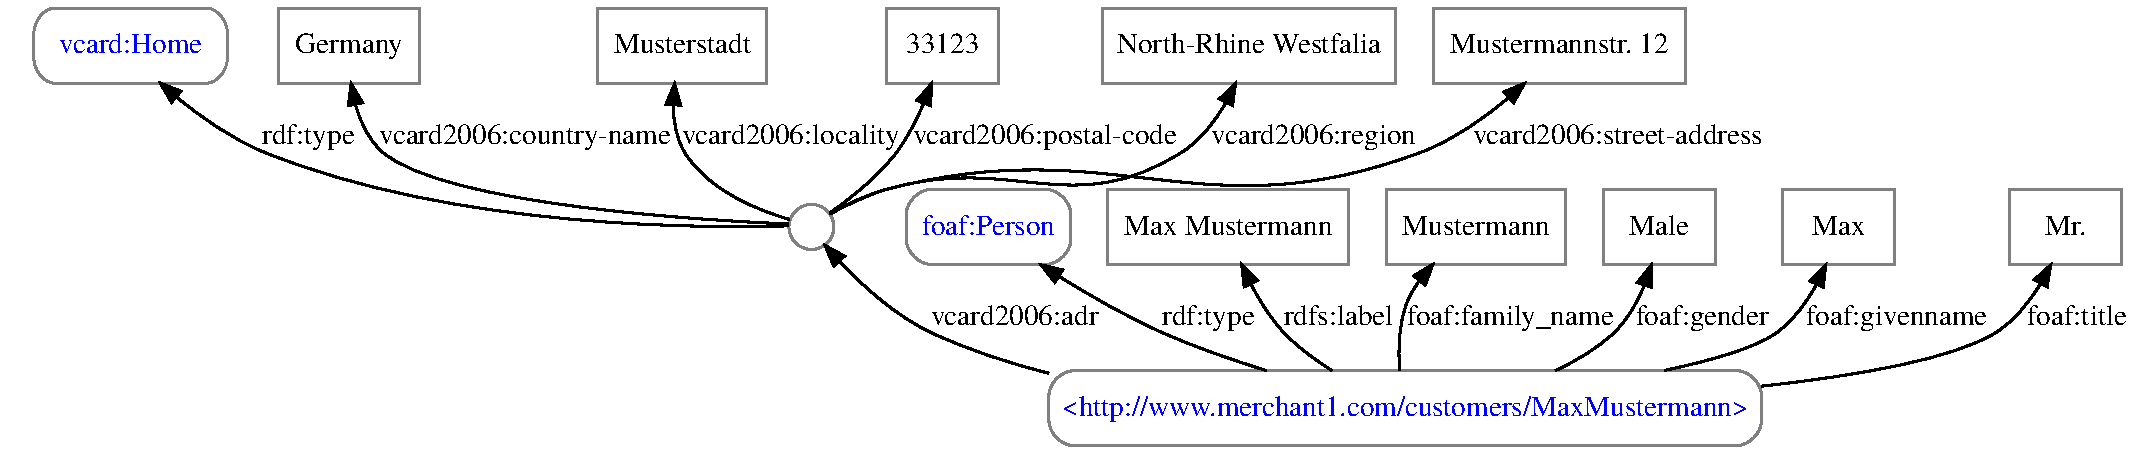
\includegraphics[width=\columnwidth]{images/sample_customer_mustermann.pdf}
	\caption{Graph representation of consumer information from Listing~\ref{lst:sample_customer_mustermann}}
\label{fig:images_sample_customer}
\end{figure}

However, being able to describe persons and their addresses is just a subset of the entities and relations found in the \gls{E-commerce} scenario. When looking back to the initial \gls{ER} model of an \gls{E-commerce} transaction as shown in Section~\ref{sec:data_model_transactions}, one can map the entities that are currently available in the \gls{E-commerce} scenario to the existing \gls{RDF} vocabularies such as follows (see Table~\ref{tab:map_tx_rdf_vocab}): \@

\begin{table}[H]
\centering
\begin{tabular}{p{5cm}l}
\hline
\textbf{Information} & \textbf{RDF vocabulary} \\
\hline
Consumer & FOAF \\
\hline
Credit Card Owner & FOAF \\
\hline
Billing Address & vCard \\
\hline
Shipping Address & vCard \\
\hline
Location Information & Geo Names \\
\hline
Merchant & GoodRelations \\
\hline
Items & GoodRelations \\
\hline
Item Categories & GoodRelations \\
\hline
Brands & GoodRelations \\
\hline
Payment Types & GoodRelations \\
\hline
\end{tabular}
\caption{Possible usage of \gls{RDF} vocabularies for \gls{E-commerce} transaction information}
\label{tab:map_tx_rdf_vocab}
\end{table}

As this table shows, there are some parts of the \gls{E-commerce} \gls{ER} model that can be expressed with existing \gls{RDF} vocabularies extensively such as personal related information via \gls{FOAF} and \gls{vCard}, whereas other parts can not be stated in-depth (e.g.\ credit card information), or are not specified at all (e.g.\ tracking of the delivery). Due to these circumstances, one usually have to build an own \gls{RDF} vocabulary or Web ontology that fills in the missing pieces, and refers to the existing concepts whenever appropriate.\\

When trying to model the information of a credit card as displayed in Figure~\ref{fig:images_data_model}, a possible result will be the \gls{RDFS} specification shown in Listing~\ref{lst:credit_card_vocab}. This definition of a credit card resource explicitly reuses entities from the \gls{FOAF} and GoodRelations ontologies by defining that: \@

\begin{itemize}
 \item the owner of a credit card has to be of type ``Person'' from the \gls{FOAF} ontology,
 \item the type of a credit card has to be an instance of the type ``PaymentMethodCreditCard'' from the GoodRelations ontology.
\end{itemize}

As most of the parts of the \gls{E-commerce} data model shown in Figure~\ref{fig:images_data_model} can not be expressed with the existing \gls{RDF} vocabularies directly, filling in the gaps would mean to come up with a large set of custom entities and relationships, which will limit the usage of the system as explained in Section~\ref{subsec:build_ontology_frauds}.

\begin{listing}[H]
 \inputminted[linenos,
              numbersep=5pt,
              breaklines=true,
              frame=lines]{TURTLE}
              {./samples/vocab_credit_card.ttl}
 \caption{A specification for a credit card in \gls{RDFS}}
\label{lst:credit_card_vocab}
\end{listing}

When analysing the list of existing and actively used \gls{RDF} vocabularies and Web ontologies in Table~\ref{tab:used_vocab_rdf}, one will also find the Schema.org initiative \citep{Schema.org}. This meta data vocabulary was initially designed by the leading search engines (e.g.\ Google, Microsoft and Yahoo!) to allow authors of Web sites to markup their \gls{HTML} documents in a way, so that they are better understood by these search engines. The Schema.org vocabulary is actively maintained by its community, includes new concepts with each release, and also offers an extension mechanism to implement additional vocabularies with terms that are not part of the core specifications \citep{SchemaExtensions} yet. In one of the past releases the maintainers also introduced all of the existing concepts of the GoodRelations ontology into the Schema.org vocabulary \citep{SchemaGoodRelation}. \\

As online merchants likely provide semantic meta data for their products and offerings in the vocabulary of Schema.org with the objective to improve their listings on search engine results (also known as \gls{SEO}) already, one can reuse parts of these information for the \gls{E-commerce} fraud investigation scenario. Additionally, the wide-ranging scope of aspects declared in the Schema.org vocabulary can make it a good fit for the collaborative system to support the investigation of \gls{E-commerce} frauds. When trying to map the initial \gls{ER} model from Section~\ref{sec:data_model_transactions} to the Schema.org core specifications, one will basically come up with a schema as displayed in Figure~\ref{fig:images_schema_org}. \@

\begin{figure}[H]
	\centering
		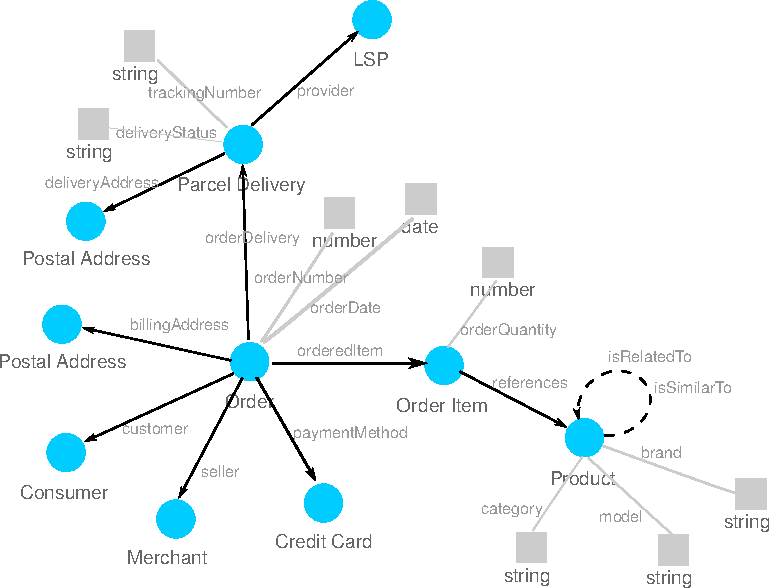
\includegraphics[width=0.8\columnwidth]{images/schema_org_mapping.pdf}
	\caption{Schema.org based mapping of an \gls{E-commerce} transaction}
\label{fig:images_schema_org}
\end{figure}

% subsection reuse_vocab_web (end)

\subsection{Creation of a custom \gls{RDF} vocabulary}
\label{subsec:build_ontology_frauds}

Another possible approach to harmonise information in the collaborative system is to define a completely new \gls{RDF} vocabulary or Web ontology for the proposed \gls{E-commerce} fraud investigation system, and share that with every possible stakeholder. This specification will have to define all the entities and relations known to the collaborative system and describe them in \gls{RDFS} format (see Section~\ref{sec:semantic_web}). \\

A major drawback of this approach is that new participants of the system will have to implement the conversion of their internal data structures to a \gls{RDF} data set that follows the predefined schema definition first, before even being able to join in. This will limit the general usage of the collaborative system, and will therefore not further considered in detail.

% subsection build ontology (end)

\subsection{Mapping of \gls{RDF} vocabularies}

Although it is possible to model an \gls{E-commerce} transaction solely with the Schema.org specifications as shown in Figure~\ref{fig:images_schema_org}, the collaborative system likely has to take care of the mapping of the transactional information coming from various sources to be able to combine them later. As the Semantic Web does not restrict how organizations structure and express their information, and due to the ``AAA slogan'' (see Section~\ref{sec:semantic_web}), there are likely different \gls{RDF} representations of an \gls{E-commerce} transaction in-use and have to be brought together. \\

The \gls{W3C} standards for the Semantic Web also include support for these mapping issues, because they will also come up when trying to combine semantic information available around the Web. The following axioms are available in the \gls{RDFS} and \gls{OWL} specifications explicitly for that purpose: \@

\begin{itemize}
	\item \textbf{rdfs:subClassOf:} a relation of type ``rdfs:subClassOf'' defines a specialization of a class, in which the child class inherits all the properties of the parent class,
  \item \textbf{rdfs:subProperyOf:} a relation of type ``rdfs:subPropertyOf'' defines a specialization of a property, in which the child property inherits all constraints of the parent property,
  \item \textbf{owl:equivalentClass:} a relation of type ``owl:equivalentClass'' specifies the equality of classes coming from different \gls{RDF} vocabularies or Web ontologies,
  \item \textbf{owl:equivalentProperty:} a relation of type ``owl:equivalentProperty'' specifies the equality of classes coming from different \gls{RDF} vocabularies or Web ontologies
\end{itemize}

If a merchant wants to state that a product related information, which is delivered as resource using the GoodRelations vocabulary, is equal to product information that can be found in the Schema.org specification, he or she can do so as follows (see Listing~\ref{lst:schema_mapping_gr_schema_org}): \@

\begin{listing}[H]
 \inputminted[linenos,
              numbersep=5pt,
              breaklines=true,
              frame=lines]{TURTLE}
              {./samples/mapping_gr_schema_org.ttl}
 \caption{Mapping product-related information from GoodRelations to Schema.org}
\label{lst:schema_mapping_gr_schema_org}
\end{listing}

These mapping statements from one \gls{RDF} vocabulary to another can be either created and injected into a \gls{RDF} data store by the party, who is going to merge information from different sources according to needs, or can also be part of the resource specification coming from an external source. In the former case the stakeholder, who is collecting and combining the information from various sources, has to maintain the additional triples to map information between each \gls{RDF} vocabulary used, and include them in the processing of the external statements within the combined \gls{RDF} data store. With an increased number of participants, which are using disjunct \gls{RDF} vocabularies, the effort and time to manage and create these mapping instructions on the collectors side will increase tremendously. Thus, the second approach is the preferred one. In that situation the \gls{RDF} description of an entity coming from an external source is already stating the mapping to one or more well-known \gls{RDF} vocabularies (e.g.\ the Schema.org specification mentioned above). This will reduce the effort and time to combine the information from different sources, and will only slightly increase the effort on the side of the external partner to prepare their internal information for external consumptions.

% subsection map ontology (end)

% sec data_schema (end)


% sub chapter combining the information
%!TEX root = ../MasterThesis.tex

\section{Combining \gls{RDF} data sets in the \gls{E-commerce} scenario}
\label{sec:working_semantic_data}

With these methods in place one can now specify how the relevant participants have to provide their information so that they can be combined and analyzed in the collaborative system. This section explains how the different participants might prepare their local context information for external consumption, and how the transactional details from various online merchants can be combined on an individual resource level to be able to analyze and cluster the transactions by different criteria as described in Section~\ref{sec:analyze_transactions}.

\subsection{Preparing internal information for external consumption}
\label{subsec:prepare_information}

As explained in Section~\ref{subsec:etl_process} there are likely \gls{ETL} processes in-use within the \gls{IT} operations of every stakeholder. These processes are usually collecting and combining information from internal data sources for \emph{internal} business analytics, but can also be used to prepare internal data for external consumption. In the latter case the parts of the relevant information for the \gls{E-commerce} fraud investigation have to be extracted from the internal databases and encoded in a \gls{RDF} data set incl. the \gls{RDFS} vocabulary used and required mapping statements to a well-known vocabulary such as the one from Schema.org as shown in Figure~\ref{fig:images_schema_org}.

\subsubsection{Merchant}
\label{subsub:prep_info_merchant}

The merchants should be able to provide \gls{RDF} encoded information for their orders based on a given payment token or based on a consumer identification. The former selector is likely used in the initial phase of collecting all required information of orders that have been done with a credit card recently. The latter one is of interest if there are malicious transactions found for a consumer and a merchant will have to provide additional order details coming from that individual. \\

The merchants provide the following information in \gls{RDF}:\@

\begin{itemize}
  \item \textbf{product-related information:} as part of the order details the merchants have detailed information about the products that have been bought by a consumer. These information include the brand, model as well as product categories of each item within an order. These are likely of interest in the \gls{E-commerce} fraud investigation. If merchants have these information in a \gls{RDFa} format on their Web sites already, they can refer to those data via the ``rdfs:seeAlso'' predicate, which holds a \gls{URI} to an external resource that contains additional information for the subject (see Listing~\ref{lst:rdfs_seeAlso_order} for an example). Additionally, the product-related information might be available in different languages on the Web shop. The merchants should use the English expression for each textual identifier in a \gls{RDF} data set and express language-dependent terms via the ``rdfs:label'' predicate that is used for a human-friendly name of the resource and supports language specifiers (see Listing~\ref{lst:rdfs_label_language} for an example).
  \item \textbf{consumer-related information:} as part of the order details the merchants also have the personal related information of the buyer incl.\ billing and shipping addresses.
  \item \textbf{merchant-related information:} the merchants can also provide information about themselves such as the retail branch they are operating in.
\end{itemize}

\begin{listing}[H]
  \inputminted[linenos,
               numbersep=5pt,
               breaklines=true,
               frame=lines]{TURTLE}
               {./samples/sample_customer_order.ttl}
  \caption[Specifying a link to a Web site for looking up product-related information in \gls{RDF}]{Specifying a link to a Web site for looking up product-related information in \gls{RDF}\protect\footnotemark}
\label{lst:rdfs_seeAlso_order}
\end{listing}

\footnotetext{Please note that the application has to resolve the \gls{URI} and embed the external \gls{RDF} data set at this position.}

\begin{listing}[H]
  \inputminted[linenos,
               numbersep=5pt,
               breaklines=true,
               frame=lines]{TURTLE}
               {./samples/sample_product_with_labels.ttl}
  \caption[Specifying a product with labels in three different languages in \gls{RDF}]{Specifying a product with labels in three different languages in \gls{RDF}\protect\footnotemark}
\label{lst:rdfs_label_language}
\end{listing}

\footnotetext{Please note that the name of the product has been stated without a language specifier, which makes it valid globally.}

\subsubsection{Payment Service Provider}
\label{subsub:prep_info_psp}

The \gls{PSP}s provide information about a payment token and the authorization request that belongs to it. These information are required to link the credit card to the order information from a merchant. Due to this the \gls{PSP}s can act as a broker between the issuers and online merchants. On the one hand they have a strong relationship with the issuers for any payment related activities, and on the other hand they have an integration of their Web service \gls{API}s at the merchants (see Section~\ref{subsec:web_services}). The benefit of this is that the issuers do not have to know about any online merchant operating on the Internet, because they can get contact information to any of these merchants from the \gls{PSP}s. In a distributed \gls{P2P} communication scenario the \gls{PSP}s can also use the \gls{RDFS} predicate ``rdfs:seeAlso'' to provide links to the affiliated online merchant of a payment authorization in their \gls{RDF} data set as shown in Listing~\ref{lst:rdfs_psp_linkto_merchant}. \@

\begin{listing}[H]
  \inputminted[linenos,
               numbersep=5pt,
               breaklines=true,
               frame=lines]{TURTLE}
               {./samples/sample_psp_linkto_merchant.ttl}
  \caption{Linking to an online merchant in the \gls{RDF} from a \gls{PSP}}
\label{lst:rdfs_psp_linkto_merchant}
\end{listing}

\subsubsection{Logistic Service Provider}
\label{subsub:prep_info_lsp}

The \gls{LSP}s provide information about a tracking number and the delivery status of an order. If the recipients have to show their ID card or have to place a signature on the delivery receipt, the \gls{LSP}s can also hand over personal related information about them. The information will be requested based on the tracking number that is shared with a merchant. In these situations the merchants will be acting as a broker between the issuers and the \gls{LSP}s due to the strong business integrations between merchants and \gls{LSP}s.

\subsubsection{Issuer}
\label{subsub:prep_info_issuer}

The issuers holds information about credit cards and their owners incl.\ personal related information. They are the ones who are usually initiating the \gls{E-commerce} fraud investigation by asking the \gls{PSP}s for detailed order information to a payment authorization request. They will also collect all the information from the different stakeholders and have to combine and analyze them to be able to validate a credit card transaction. To be able to do so they will have to use a \gls{RDF} data store, in which the dispersed \gls{RDF} data sets are imported and linked against each other (see next section).

\subsection{Merging transactional information from various sources}
\label{subsec:information_mapping}

Still, if the transactional details from various online merchants have to be linked together on the individual entity level to support analyzing and clustering the information on different aspects, the build-in merging capabilities of the \gls{RDF} specification will rely on unique \gls{URI}s used for the same entities found in different \gls{RDF} data sets as shown in the Section~\ref{subsec:web_data}. These unique \gls{URI}s are used to identify the resources in a dispersed \gls{RDF} data set. \@

\begin{itemize}
	\item \textbf{owl:sameAs, schema:sameAs}: the ``owl:sameAs'' as well as the ``schema:sameAs'' relations are providing an unique \gls{URI} that unambiguously define the subject (see Listing~\ref{lst:schema_sameAs_location} for an example)
\end{itemize}

\begin{listing}[H]
  \inputminted[linenos,
               numbersep=5pt,
               breaklines=true,
               frame=lines]{TURTLE}
               {./samples/sample_customer_location.ttl}
  \caption{Specifying a link to a DBpedia resource to uniquely identify an entity in \gls{RDF}}
\label{lst:schema_sameAs_location}
\end{listing}

When looking at the \gls{E-commerce} transaction schema as defined in Section~\ref{sec:data_model_transactions} the following information must be uniquely identified and mapped within the \gls{RDF} data sets coming from the participants of the collaborative system: \@

\begin{itemize}
	\item \textbf{personal related information} such as the consumer, recipient and credit card owner
	\item \textbf{location based information} such as the billing and shipping address as well as the location a credit card owner is registered for
	\item \textbf{product related information} such as the categories, subcategories, brand, model and item description
	\item \textbf{merchant related information} such as the branch of a merchant
\end{itemize}

To support the unique identification of entities in the \gls{RDF} data set of an \gls{E-commerce} transaction, one can refer to publicly available \gls{RDF} data sets on the Internet, such as GeoNames or DBpedia. These can provide an unique \gls{URI} for locations and named places. A product-related \gls{RDF} data set was available in form of the ProductDB initiative until recently \citep{bouzidi2014product}. Due to the shutdown of it, the mapping of products can no longer be done by referencing unique \gls{URI}s from the Web, but will have to be based on the global trade item number (aka \gls{GTIN}) of each product. Additional aspects of an item, such as brand, categories and subcategories, can be found on DBpedia as well. \\

A problem, that will come up, is the unique addressing of personal related information, such as identifying the consumer. The collaborative system can not rely on mapping the personal related information based on properties such as familyName and givenName alone (see Listing~\ref{lst:sample_customer_mustermann}). There could be typos in the information coming from various \gls{RDF} data sets, and different individuals can still have the same name information. One possible approach to bring these information together would be the mapping based on the e-mail address of the individual. An e-mail address like an \gls{URI} is a globally unique addressing scheme, and one can assume that two entities, who are using to the same e-mail address, are referring to the same entity. Still this is only a weak hint as an individual can have more than one e-mail address, and could use different e-mail addresses for the online shopping trips at different merchants. Therefore a more sophisticated mapping algorithm for personal related information is needed in the collaborative system. This algorithm may take into account the combination of familyName, givenName, dateOfBirth as well as location-based information to uniquely identify an individual. To sum up, the identification of important entities from an \gls{E-commerce} transaction can be based on the following aspects (see Table~\ref{tab:mapping_information}): \@

\begin{table}[H]
\centering
\begin{tabular}{lllp{4cm}}
\hline
\textbf{Entity} & \textbf{Unique Identifier} & \textbf{Public Data Set} & \textbf{Example} \\
\hline
Person & eventually e-Mail address & n/a & \url{mailto:max.mustermann@t-online.de} \\
\hline
PostalAddress & Location, Position & Geo Names & \url{http://sws.geonames.org/2886242/} \\
\hline
Item & \gls{GTIN}, \gls{ISBN} & n/a & \url{gtin:9781617290398} \\
\hline
Brand & Name & DBpedia & \url{http://dbpedia.org/resource/Samsung} \\
\hline
Organization & Web Site \gls{URL} & n/a & \url{http://www.samsung.com} \\
\hline
\end{tabular}
\caption{List of possible criteria to uniquely identify entities of an \gls{E-commerce} transaction}
\label{tab:mapping_information}
\end{table}

% subsec information_mapping (end)

% sec provide_information (end)


% sub chapter the p2p communication system
%!TEX root = ../MasterThesis.tex

\section{A partially centralized \gls{P2P} system proposal}
\label{sec:p2p_partially_centralized_system}

In the \gls{E-commerce} fraud scenario, which has been selected for this Master Thesis in Section~\ref{sec:scope_thesis}, the issuer of a credit card is the participant, who initiates a collaborative session to investigate a suspicious online transaction. Issuers are recognizing the active use (and maybe misuse) of a credit card in the online and the offline world first, and are also getting notifications about any suspicious activity from their fraud prevention systems. Due to these circumstances, a valid design proposal for the \gls{E-commerce} fraud investigation system is based on a partially centralized \gls{P2P} communication network, in which the issuer of a credit card is taking over a leading position.

\subsection{Role of the issuer}
\label{subsec:p2p_partially_issuer_collecting}

In case a suspicious activity has been detected by the fraud prevention system of an issuer, one of their investigators will initiate a collaborative session with the relevant stakeholders that have been selected based on the usage history of the credit card in question. To establish the \gls{P2P} communication session, the investigator creates a new \gls{WebRTC} communication session in the collaborative system, which has been implemented as a Web application. By doing so, the investigator receives a unique session ID that can be transmitted to merchants, \gls{PSP}s and \gls{LSP}s, so that they can join the session in the collaborative system. As the investigator is just being aware of the \gls{PSP}s affected, they can invite them directly due to the existing business relationship between both parties. Based on the given credit card information, the \gls{PSP}s can relate each payment authorization request to an order of an online merchant by referring to the payment authorization token. So the \gls{PSP}s will know the merchants that have to be involved in this \gls{E-commerce} fraud investigation, and can hand over contact information to the issuer for inviting them. Each online merchant can do likewise with the \gls{LSP} that has been used to handle the delivery of an order via the tracking number (as depicted in Figure~\ref{fig:system_workflow}). \\

As soon as the relevant merchants, \gls{PSP}s and \gls{LSP}s have joined the \gls{P2P} communication session, they will start sharing their information with the issuer. The information exchanged have been prepared as \gls{RDF} data sets by internal \gls{ETL} processes, and has been made available to the support staff of each stakeholder. During the information sharing process the \gls{RDF} data sets of each stakeholder are replicated to the issuer, who will do the mapping and linking into a combined \gls{RDF} data store locally (as described in Section~\ref{sec:working_semantic_data}). This combination of the dispersed \gls{RDF} data sets will take place in a \gls{RDF} data store that the issuers have to setup and operate within their organization. Parts of this \gls{RDF} data store will take care of the reasoning over the merged \gls{RDF} data set to infer additional triple statements, as well as provide an internal \gls{SPARQL} endpoint to query the data store from the Web application as shown in Figure~\ref{fig:images_semweb_app}. \\

Thus, the major tasks will be done on the side of the issuers, which are coordinating and executing the \gls{E-commerce} fraud investigations as depicted in Figure~\ref{fig:images_p2p_centralized}.\@

\begin{figure}[H]
	\centering
		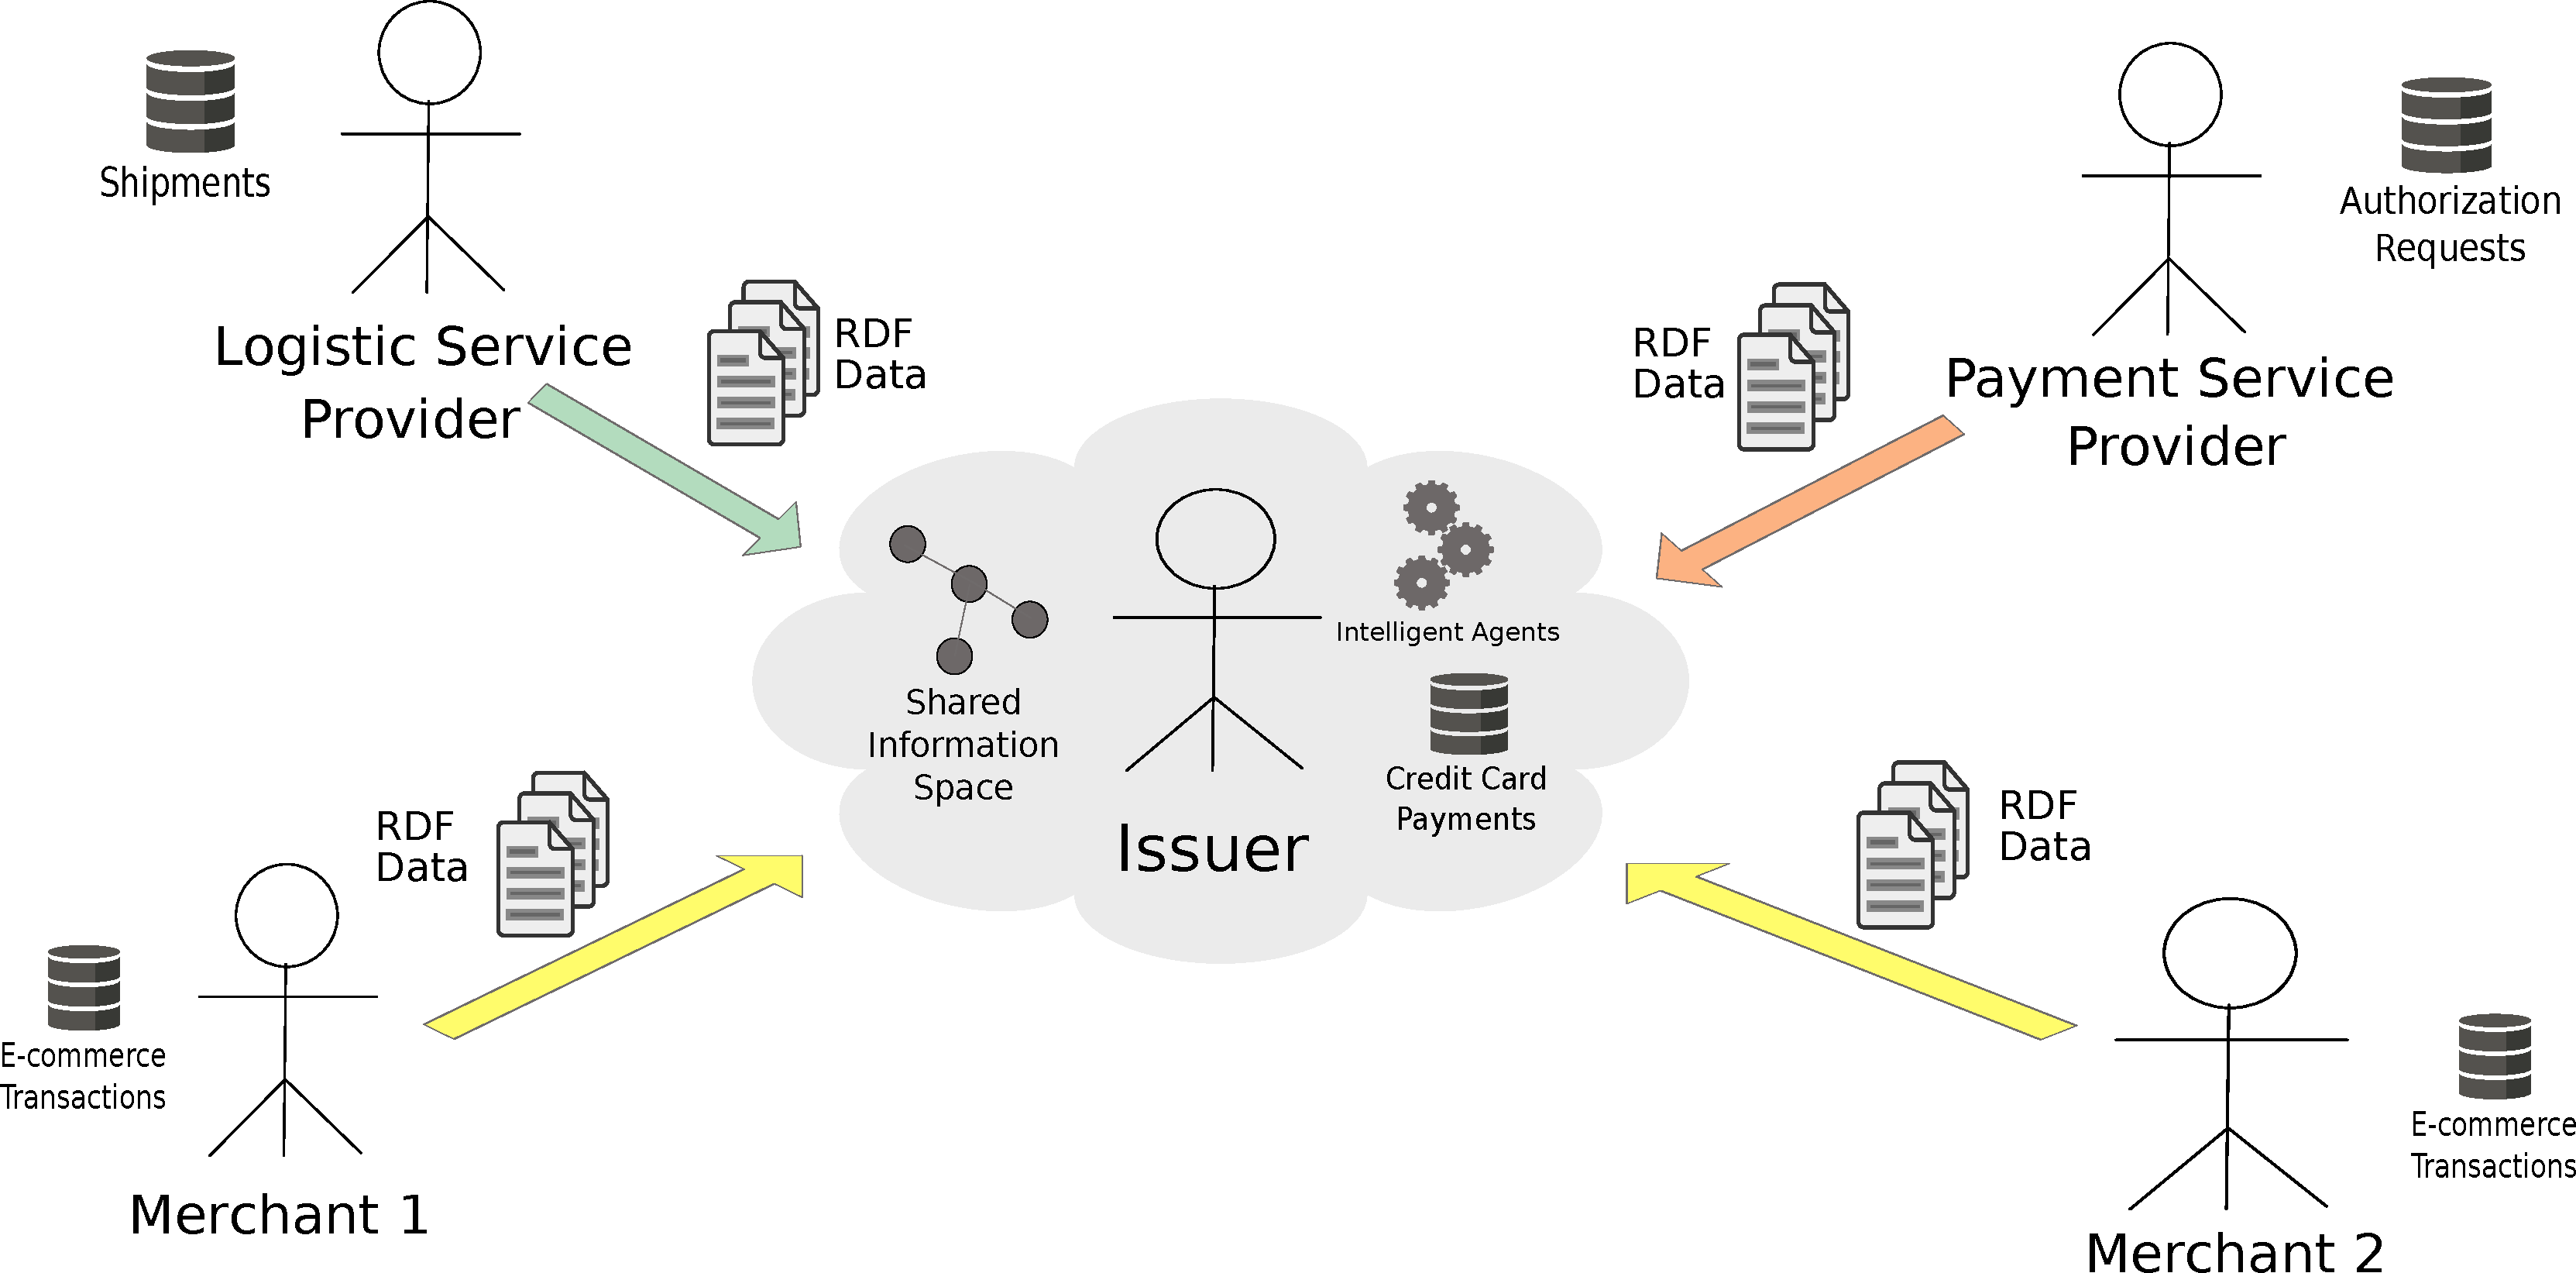
\includegraphics[width=0.9\columnwidth]{images/system_P2P_centralized.pdf}
	\caption{Collaborative system using a partially centralized \gls{P2P} architecture}
\label{fig:images_p2p_centralized}
\end{figure}


\subsection{Handling of privacy issues}
\label{subsec:p2p_partially_issuer_privacy}

One of the major concerns with the system architecture mentioned above is that the merchants, \gls{PSP}s and \gls{LSP}s have to hand over all of their relevant information to the issuer of a credit card for analysing the \gls{E-commerce} activities of a consumer. This can raise severe privacy issues, because an issuer will receive a lot of detailed order information from the other parties within this collaborative system. Issuers can not only use these information for validating the correctness of suspicious online transactions, but can also misuse them to build elaborate consumer profiles, which can directly influence the scoring of that consumer in the internal credit and risk rating systems of the issuers. \\

In addition to that, online merchants will likely not provide to much detail information about their sales and offerings in such a collaborative system, because direct competitors might also be involved in the \gls{E-commerce} fraud investigation. By sharing parts of the business relevant information, the merchants will raise the fear that their internal business processes, pricing structures, as well as customer loyalty activities get more transparent to their competitors, which might lead to a stronger competition afterwards. \\

During the design of the collaborative system a valuation of the shared information has to take place, which classify each of them based on the criteria: \@

\begin{itemize}
	\item Is the information really necessary to evaluate the \gls{E-commerce} transactions? Some of the order details from the merchants might not be required to analyse the transactions with the objective to find out about abnormal behaviours.
	\item Is the information worth protecting? Parts of the necessary information are sensitive information and should be protected against misuse.
\end{itemize}

Special considerations have to be taken for mandatory \emph{and} sensitive information. In that case, cryptographic algorithms such as hash functions (e.g.\ \gls{SHA-2}) can be used to anonymise the information. A hash function is working in one-direction only, and generates a unique hash value based on its input parameter. This hash value is different as soon as the input changes only slightly, and due to the mathematical algorithms used for computing it, a hash value can not be calculated back to the original input value of the hash function afterwards. \\

A valid use case for such a hashing of information is the e-mail address of a consumer. A plaintext e-mail address such as ``max.mustermann@web.de'' will always result in a \gls{SHA-2}56 based hash value of ``349124ca834949537d726da26dc029e593be72a8b00b81 c47124f5d009c9982b'' regardless of the stakeholder, who has originally computed it. That is an additional benefit of the usage of hash functions, because they still allow the information from different stakeholders to be linked together based on their unique hash values. \\

Another approach to protect sensitive information is to consolidate them in a broader context --- a process called data generalization. An example for that would be the item categories, which can be split up into multiple hierarchical layers to narrowly define the affiliations of items to certain product groups. Instead of exchanging item descriptions with the complete set of categories they belong to, merchants can just share items and their top n categories to obfuscate detailed information about the products bought by a consumer. The same approach will also work for location based information, in which the shared information will not contain the exact geographic position from the original data set, but use an approximation to it by stating locations on a broader scope (e.g.\ district, city or region) instead. \\

Based on these explanations the information, which is shared in the \gls{E-commerce} fraud investigation, can be classified into one of the following four quadrants, and should be handled as depicted in Figure~\ref{fig:images_handle_privacy_concerns}. \@

\begin{figure}[H]
	\centering
		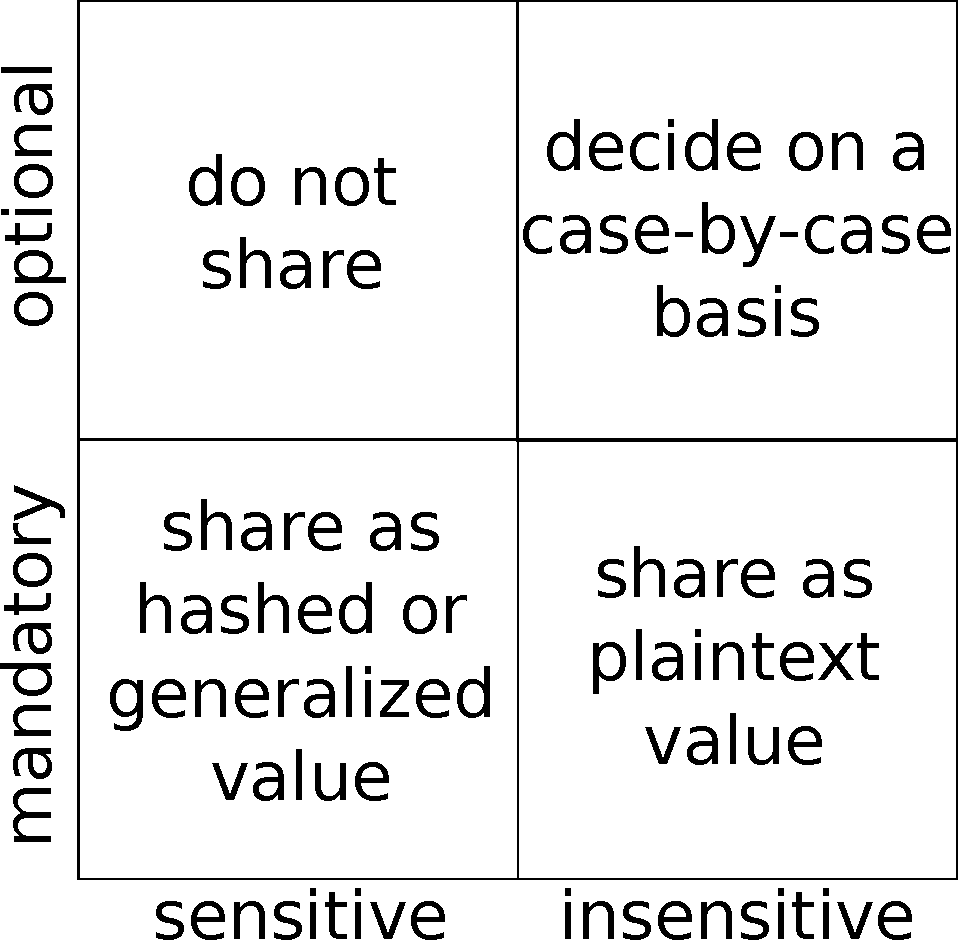
\includegraphics[width=0.5\columnwidth]{images/privacy_concerns.pdf}
	\caption{Privacy related classification of information in the collaborative system}
\label{fig:images_handle_privacy_concerns}
\end{figure}

% subsec p2p_partially_centralized_system

% section design_proposal (end)


% chapter design system (end)
